\section*{Appendices}
\vspace{1.6ex}
\titlecontents{psection}[2.3em]{}{\contentslabel{2.3em}}{}{\titlerule*[1pc]{.}\contentspage}
\startcontents[sections]
\printcontents[sections]{p}{1}{\setcounter{tocdepth}{2}}
\clearpage

\section{Benchmark Overview}
\begin{table}[h!]
\centering
\begin{mytabular}{
  colspec = {| L{6em} | C{3.5em} C{3.5em} C{3.5em} C{3.5em} C{3.5em} C{3.5em} C{3.5em} |},
  row{1} = {font=\bfseries},
}

\toprule
\newline Benchmark & \newline Tasks & Env Steps & Action Repeat & Env \llap{I}nstances & Train Ratio & GPU Days & Model Size \\
\midrule
DMC Proprio & 18 & 500K & 2 &  4 &  512 & \o\llap{<}1 & S \\
DMC Vision  & 20 &   1M & 2 &  4 &  512 & \o\llap{<}1 & S \\
Crafter     &  1 &   1M & 1 &  1 &  512 &         \o2 & XL \\
BSuite      & 23 &  --- & 1 &  1 & 1024 & \o\llap{<}1 & XL \\
Atari 100K  & 26 & 400K & 4 &  1 & 1024 & \o\llap{<}1 & S \\
Atari 200M  & 55 & 200M & 4 &  8 &   64 &          16 & XL \\
DMLab       &  8 &  50M & 4 &  8 &   64 &         \o4 & XL \\
Minecraft   &  1 & 100M & 1 & 16 &   16 &          17 & XL \\
\bottomrule

\end{mytabular}
\caption{Benchmark overview. The train ratio is the number of replayed steps per policy steps rather than environment steps, and thus unaware of the action repeat. BSuite sets the number of episodes rather than env steps, both of which vary across tasks. BSuite requires multiple configurations per environment and one seed per configuration, resulting in 468 runs. For DMC, the proprioceptive benchmark excludes the quadruped tasks that are present in the visual benchmark because of baseline availability in prior work. All agents were trained on 1 Nvidia V100 GPU each.}
\label{tab:benchmarks}
\end{table}

\section{Model Sizes}
\begin{table}[h!]
\centering
\begin{mytabular}{
  colspec = {| L{10em} | C{4.5em} C{4.5em} C{4.5em} C{4.5em} C{4.5em} |},
  row{1} = {font=\bfseries},
}

\toprule
Dimension & XS & S & M & L & XL \\
\midrule
GRU recurrent units  & 256 & 512 & 1024 & 2048 & 4096 \\
CNN multiplier  &  24 &  32 &   48 &   64 &   96 \\
Dense hidden units & 256 & 512 &  640 &  768 & 1024 \\
MLP layers &   1 &   2 &    3 &    4 &    5 \\
\midrule
Parameters & 8M & 18M & 37M & 77M & 200M \\
\bottomrule

\end{mytabular}
\caption{Model sizes. The encoder consists of stride 2 convolutions of doubling depth until resolution $4\times4$ followed by flattening. The decoder starts with a dense layer, followed by reshaping to $4\times4\times C$ and then inverts the encoder architecture. The dynamics are implemented as RSSM with vectors of categorical representations, consisting of a GRU and dense layers.}
\label{tab:models}
\end{table}
\clearpage

\newgeometry{top=1.5cm,bottom=2cm,left=2cm,right=2cm,footskip=14pt}
\section{Summary of Differences}
\label{sec:diff}

DreamerV3 builds upon the DreamerV2 algorithm \citep{hafner2020dreamerv2}. This section describes the main changes that we applied in order to master a wide range of domains with fixed hyperparameters and enable robust learning on unseen domains.

\begin{itemize}
\itempar{Symlog predictions} We symlog encode inputs to the world model and use symlog predictions with squared error for reconstructing inputs. The reward predictor and critic use twohot symlog predictions, a simple form of distributional reinforcement learning \citep{bellemare2017c51}.
\itempar{World model regularizer} We experimented with different approaches for removing the need to tune the KL regularizer, including targeting a fixed KL value. A simple yet effective solution turned out to combine KL balancing that was introduced in DreamerV2 \citep{hafner2020dreamerv2} with free bits \citep{kingma2016freebits} that were used in the original Dreamer algorithm \citep{hafner2019dreamer}. GECO \citep{rezende2018geco} was not useful in our case because what constitutes ``good'' reconstruction error varies widely across domains.
\itempar{Policy regularizer} Using a fixed entropy regularizer for the actor was challenging when targeting both dense and sparse rewards. Scaling large return ranges down to the $[0, 1]$ interval, without amplifying near-zero returns, overcame this challenge. Using percentiles to ignore outliers in the return range further helped, especially for stochastic environments. We did not experience improvements from regularizing the policy towards its own EMA \citep{hilton2021ewmappo} or the CMPO regularizer \citep{hessel2021muesli}.
\itempar{Unimix categoricals} We parameterize the categorical distributions for the world model representations and dynamics, as well as for the actor network, as mixtures of 1\% uniform and 99\% neural network output \citep{wiering1999unimix,gruslys2017reactor} to ensure a minimal amount of probability mass on every class and thus keep log probabilities and KL divergences well behaved.
\itempar{Architecture} We use a similar network architecture but employ layer normalization \citep{ba2016layernorm} and SiLU \citep{hendrycks2016silu} as the activation function. For better framework support, we use same-padded convolutions with stride 2 and kernel size 3 instead of valid-padded convolutions with larger kernels. The robustness of DreamerV3 allowed us to use large networks that contributed to its performance.
\itempar{Critic EMA regularizer} We compute $\lambda$-returns using the fast critic network and regularize the critic outputs towards those of its own weight EMA instead of computing returns using the slow critic. However, both approaches perform similarly in practice.
\itempar{Replay buffer} DreamerV2 used a replay buffer that only replays time steps from completed episodes. To shorten the feedback loop, DreamerV3 uniformly samples from all inserted subsequences of size batch length regardless of episode boundaries.
\itempar{Hyperparameters} The hyperparameters of DreamerV3 were tuned to perform well across both the visual control suite and Atari 200M at the same time. We verified their generality by training on new domains without further adjustment, including Crafter, BSuite, and Minecraft.
\end{itemize}

\subsection*{Target Regularizers}

We also experimented with constrained optimization for the world model and policy objectives, where we set a target value that the regularizer should take on, on average across states.
We found combining this approach with limits on the allowed regularizer scales to perform well for the world model, at the cost of additional complexity.
For the actor, choosing a target randomness of $40\%$---where $0\%$ corresponds to the most deterministic and $100\%$ to the most random policy---learns robustly across domains but prevents the policy from converging to top scores in tasks that require speed or precision and slows down exploration under sparse rewards.
The solutions in DreamerV3 do not have these issues intrinsic to constrained optimization formulations.

\restoregeometry
\clearpage

\newgeometry{top=2cm,bottom=1.8cm,left=2.5cm,right=2.5cm}
\section{Ablation Curves}
\begin{figure}[h]
\centering
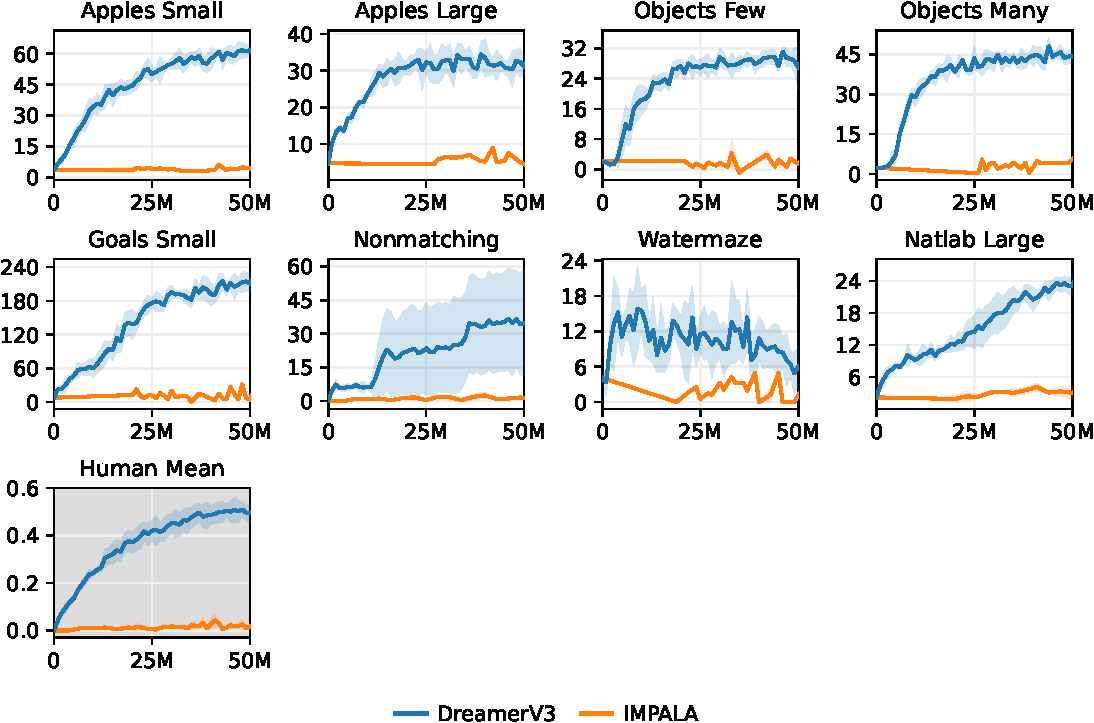
\includegraphics[width=1\linewidth]{dmlab/dmlab}
\caption{DMLab scores with a budget of 50M frames. Separate agents were trained for each task, corresponding to the IMPALA Experts method in \citet{espeholt2018impala}. Data efficiency is not the goal of IMPALA and it might be possible to tune it for improved data efficiency. Longer training curves and asymptotic performance of IMPALA are included in \cref{sec:dmlab_eff}.}
\label{fig:dmlab}
\end{figure}
\restoregeometry
\clearpage
\newgeometry{top=1.5cm,bottom=2cm,left=2cm,right=2cm,footskip=14pt}

\section{Ablation Explanation}

\subsection*{World Model Ablations}

\paragraph{NoFreeBits} Use KL balancing but no free bits, equivalent to setting the constants in \cref{eq:wm} from 1 to 0. This objective was used in DreamerV2 \citep{hafner2020dreamerv2}.
\paragraph{NoKLBalance} Use free bits but no KL balancing by setting $\beta_{\mathrm{dyn}} = \beta_{\mathrm{dyn}} = 0.5$, which recovers the $\beta$-VAE objective \citep{higgins2016beta}. We found this value to perform well compared to nearby values. This objective was used in the first Dreamer agent \citep{hafner2019dreamer}.
\paragraph{NoObsSymlog} This ablation removes the symlog encoding of inputs to the world model and also changes the symlog MSE loss in the decoder to a simple MSE loss. Because symlog encoding is only used for vector observations, this ablation is equivalent to DreamerV3 on purely image-based environments.
\paragraph{TargetKL} Target a KL value of 3.5 nats on average over the replay buffer by increasing or decreasing the KL scale (both $\beta_{\mathrm{pred}}$ and $\beta_{\mathrm{rep}}$) by 10\% when the batch average of the KL value exceeds or falls below the tolerance of 10\% around the target value, similar to the KL-penalty variant of PPO \citep{schulman2017ppo}. The KL scale is limited to the range $[10^{-3}, 1.0]$ for numerical stability.

\subsection*{Critic Ablations}

\paragraph{RewardNorm} Instead of normalizing rewards, normalize rewards by dividing them by a running standard deviation and clipping them beyond a magnitude of 10.
\paragraph{ContRegression} Using MSE symlog predictions for the reward and value heads.
\paragraph{SqrtTransform} Using two-hot discrete regression with the asymmetric square root transformation introduced by R2D2 \citep{kapturowski2018r2d2} and used in MuZero \citep{schrittwieser2019muzero}.
\paragraph{SlowTarget} Instead of using the fast critic for computing returns and training it towards the slow critic, use the slow critic for computing returns \citep{mnih2015dqn}.

\subsection*{Actor Ablations}

\paragraph{NoDenomMax} Normalize returns directly based on the range between percentiles 5 to 95 with a small epsilon in the denominator, instead of by the maximum of 1 and the percentile range. This way, not only large returns are scaled down but also small returns are scaled up.
\paragraph{AdvantageStd} Advantage normalization as commonly used, for example in PPO \citep{schulman2017ppo} and Muesli \citep{hessel2021muesli}. However, scaling advantages without also scaling the entropy regularizer changes the trade-off between return and entropy in a way that depends on the scale of advantages, which in turn depends on how well the critic currently predicts the returns.
\paragraph{ReturnStd} Instead of normalizing returns by the range between percentiles 5 to 95, normalize them by their standard deviation. When rewards are large but sparse, the standard deviation is small, scaling up the few large returns even further.
\paragraph{TargetEntropy} Target a policy randomness of 40\% on average across imagined states by increasing or decreasing the entropy scale $\eta$ by 10\% when the batch average of the randomness falls below or exceeds the tolerance of 10\% around the target value. The entropy scale is limited to the range $[10^{-3}, 3\cdot10^{-2}]$. Policy randomness is the policy entropy mapped to range from 0\% (most deterministic allowed by action distribution parameterization) to 100\% (most uniform). Multiplicatively, instead of additively, adjusting the regularizer strength allows the scale to quickly move across orders of magnitude, outperforming the target entropy approach of SAC \citep{haarnoja2018sac} in practice. Moreover, targeting a randomness value rather than an entropy value allows sharing the hyperparameter across domains with discrete and continuous actions.

\restoregeometry
\clearpage

\newgeometry{top=1.5cm,bottom=2cm,left=2cm,right=2cm,footskip=14pt}

\section{Minecraft Environment}
\label{sec:mcenv}

\paragraph{Minecraft}
With 100M monthly active users, Minecraft is one of the most popular video games worldwide.
Minecraft features a procedurally generated 3D world of different biomes, including plains, forests, jungles, mountains, deserts, taiga, snowy tundra, ice spikes, swamps, savannahs, badlands, beaches, stone shores, rivers, and oceans.
The world consists of 1 meter sized blocks that the player and break and place.
There are about 30 different creatures that the player can interact and fight with.
From gathered resources, the player can use 379 recipes to craft new items and progress through the technology tree, all while ensuring safety and food supply to survive.
There are many conceivable tasks in Minecraft and as a first step, the research community has focused on the salient task of obtaining a diamonds, a rare item found deep underground and requires progressing through the technology tree.

\paragraph{Environment}
We built the Minecraft Diamond environment on top of MineRL to define a flat categorical action space and fix issues we discovered with the original environments via human play testing.
For example, when breaking diamond ore, the item sometimes jumps into the inventory and sometimes needs to be collected from the ground.
The original environment terminates episodes when breaking diamond ore so that many successful episodes end before collecting the item and thus without the reward.
We remove this early termination condition and end episodes when the player dies or after 36000 steps, corresponding to 30 minutes at the control frequency of 20Hz.
Another issue is that the jump action has to be held for longer than one control step to trigger a jump, which we solve by keeping the key pressed in the background for 200ms.
We built the environment on top of MineRL v0.4.4 \citep{guss2019minerl}, which offers abstract crafting actions. The Minecraft version is 1.11.2.

\paragraph{Rewards}
We follow the same sparse reward structure of the MineRL competition environment that rewards 12 milestones leading up to the diamond, namely collecting the items log, plank, stick, crafting table, wooden pickaxe, cobblestone, stone pickaxe, iron ore, furnace, iron ingot, iron pickaxe, and diamond.
The reward for each item is only given once per episode, and the agent has to learn autonomously that it needs to collect some of the items multiple times to achieve the next milestone. 
To make the return curves easy to interpret, we give a reward of $+1$ for each milestone instead of scaling rewards based on how valuable each item is.
Additionally, we give a small reward of $-0.01$ for each lost heart and $+0.01$ for each restored heart, but we did not investigate whether this was helpful.

\paragraph{Inputs}
The sensory inputs include the $64\times64\times3$ RGB first-person camera image, the inventory counts as a vector with one entry for each of the game's over 400 items, the vector of maximum inventory counts since episode begin to tell the agent which milestones it has already achieved, a one-hot vector indicating the equipped item, and scalar inputs for the health, hunger, and breath levels.

\paragraph{Actions}
The MineRL environment provides a dictionary action space and delegates choosing a simple action space to the user. We use a flat categorical action space with 25 actions for walking in four directions, turning the camera in four directions, attacking, jumping, placing items, crafting items near a placed crafting table, smelting items near a placed furnace, and equipping crafted tools. Looking up and down is restricted to the range $-60$ to $+60$ degrees. The action space is specific to the diamond task and does not allow the agent to craft all of the 379 recipes. For multi-task learning, a larger factorized action space as available in MineDojo \citep{fan2022minedojo} would likely be beneficial.

\paragraph{Break Speed Multiplier}
We follow \citet{kanitscheider2021minecraftcurriculum} in allowing the agent to break blocks in fewer time steps.
Breaking blocks in Minecraft requires holding the same key pressed for sometimes hundreds of time steps.
Briefly switching to a different key will reset this progress.
Without an inductive bias, stochastic policies will almost never sample the same action this often during exploration under this parameterization.
To circumvent this issue, we set the break speed multiplier option of MineRL to 100.
In the future, inductive biases such as learning action repeat as part of the agent \citep{park2021timeinvariantpg} could overcome this caveat.

\restoregeometry
\clearpage

\section{Minecraft Item Rates}

Across 40 seeds trained for 100M steps, DreamerV3 obtained the maximum episode score---that includes collecting at least one diamond---50 times. It achieves this score the first time at 29.3M steps and as expected the frequency increases over time. Diamonds can also rarely be found by breaking village chests, but those episodes do not achieve the maximum score and thus are not included in this statistic.
A total of 24 out of 40 seeds achieve the maximum episode score at least once, and the most successful seed achieved the maximum score 6 times. Across all seeds, the median number of environment steps until collecting the first diamond is 74M, corresponding to 42 days of play time at 20 Hz.

\begin{figure}[h]
\centering
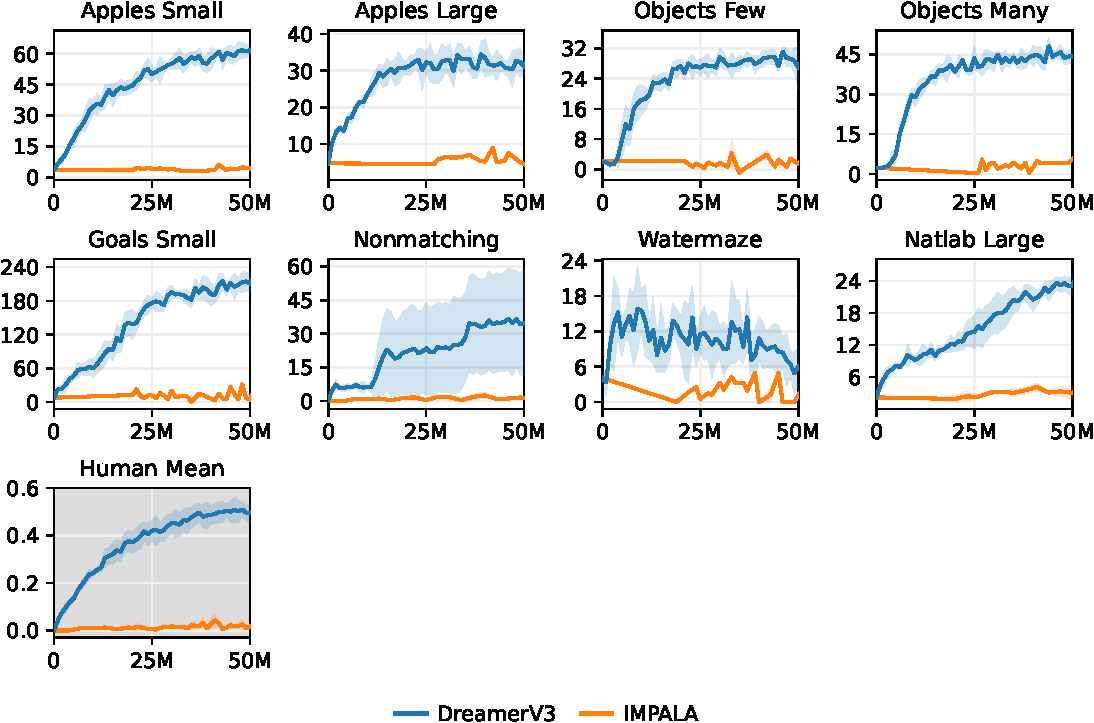
\includegraphics[width=1\linewidth]{dmlab/dmlab}
\caption{DMLab scores with a budget of 50M frames. Separate agents were trained for each task, corresponding to the IMPALA Experts method in \citet{espeholt2018impala}. Data efficiency is not the goal of IMPALA and it might be possible to tune it for improved data efficiency. Longer training curves and asymptotic performance of IMPALA are included in \cref{sec:dmlab_eff}.}
\label{fig:dmlab}
\end{figure}
\clearpage

\newgeometry{top=2cm,bottom=2cm,left=3cm,right=3cm}
\section{Minecraft Video Predictions}
\label{sec:openl}
\begin{figure}[ht!]
\centering
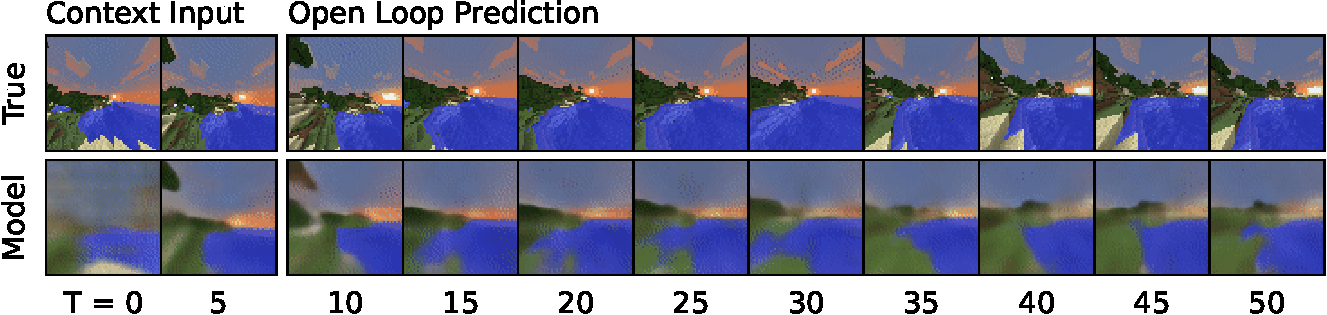
\includegraphics[width=\linewidth,trim={0 .5cm 0 0},clip]{openl/mine1} \\[1ex]
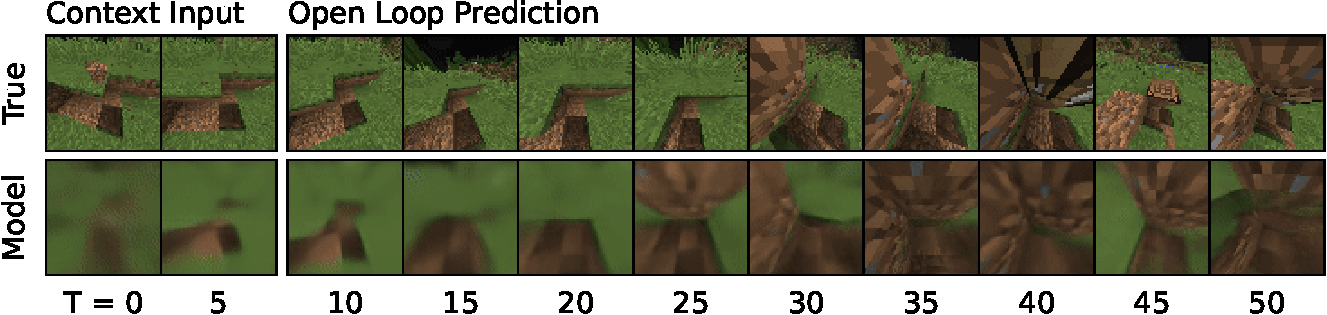
\includegraphics[width=\linewidth,trim={0 .5cm 0 .5cm},clip]{openl/mine2} \\[1ex]
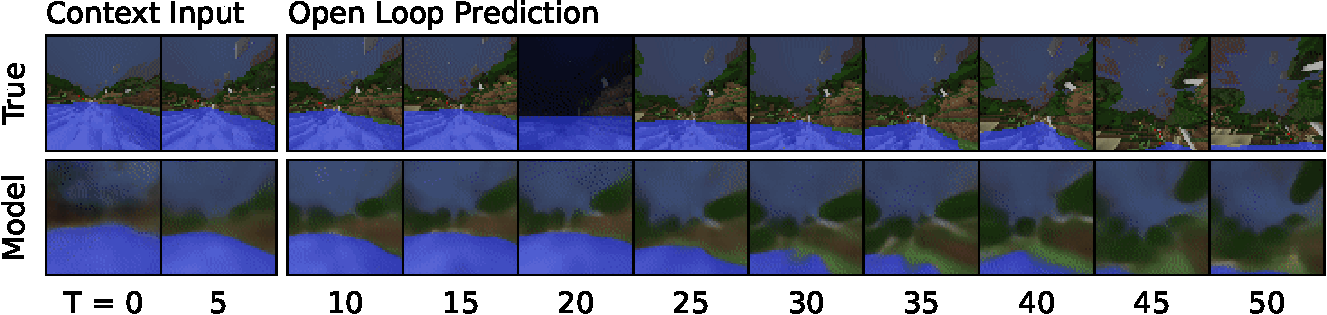
\includegraphics[width=\linewidth,trim={0 .5cm 0 .5cm},clip]{openl/mine3} \\[1ex]
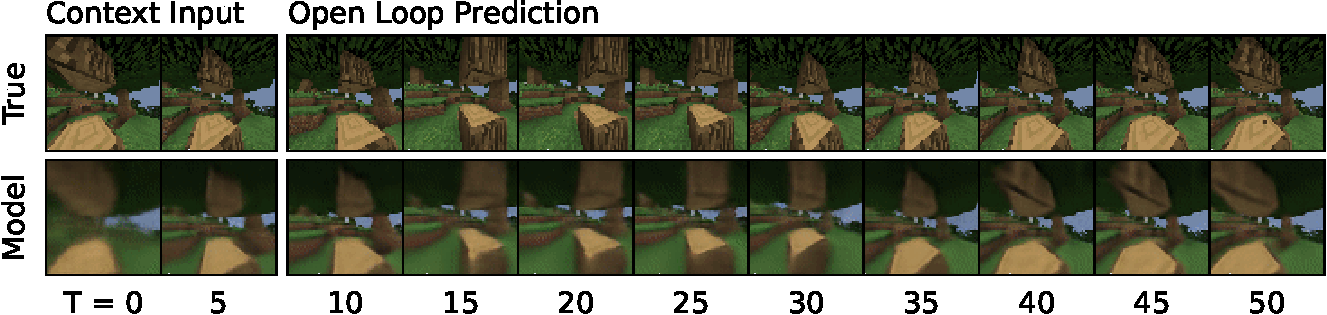
\includegraphics[width=\linewidth,trim={0 .5cm 0 .5cm},clip]{openl/mine4} \\[1ex]
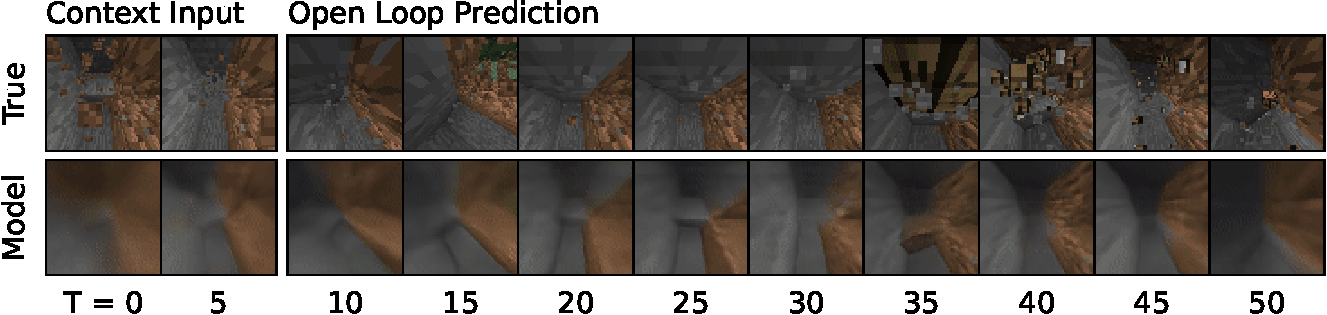
\includegraphics[width=\linewidth,trim={0 .5cm 0 .5cm},clip]{openl/mine5} \\[1ex]
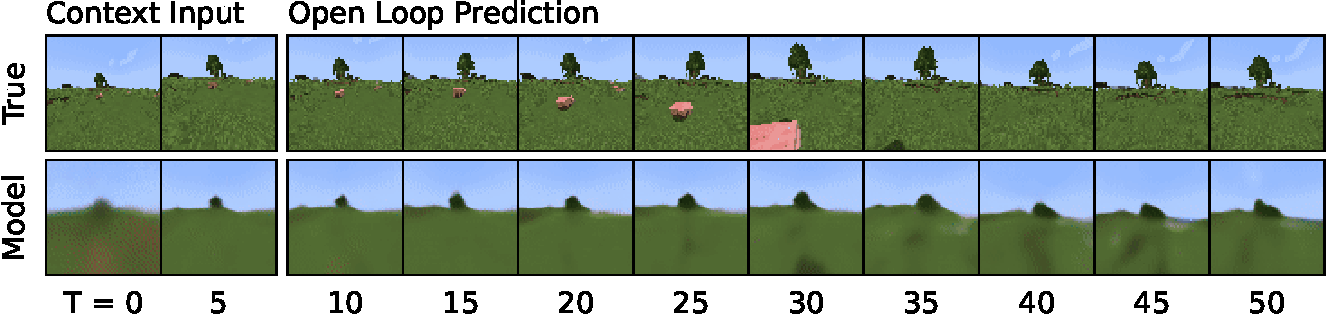
\includegraphics[width=\linewidth,trim={0 0 0 .5cm},clip]{openl/mine6} \\[1ex]
\caption{Multi-step predictions on Minecraft. The model receives the first 5 frames as context input and the predicts 45 steps into the future given the action sequence and without access to intermediate images.}
\label{fig:openl_more}
\end{figure}

\restoregeometry
\clearpage

\newgeometry{top=1.5cm,bottom=1.5cm,left=2.5cm,right=2.5cm}
\section{DMLab Curves}
\vspace*{-1ex}
\begin{figure}[h]
\centering
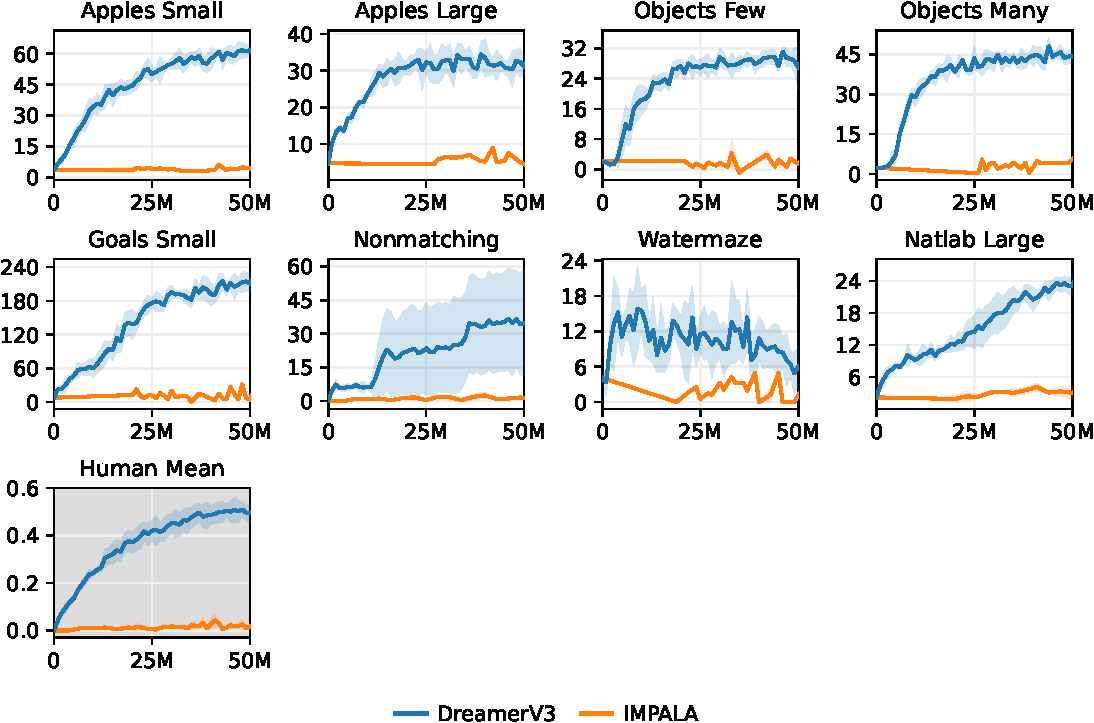
\includegraphics[width=1\linewidth]{dmlab/dmlab}
\caption{DMLab scores with a budget of 50M frames. Separate agents were trained for each task, corresponding to the IMPALA Experts method in \citet{espeholt2018impala}. Data efficiency is not the goal of IMPALA and it might be possible to tune it for improved data efficiency. Longer training curves and asymptotic performance of IMPALA are included in \cref{sec:dmlab_eff}.}
\label{fig:dmlab}
\end{figure}
\vspace*{-2ex}
\section{DMLab Scores}
\vspace*{-2ex}
\begin{table*}[h!]
\centering
\begin{mytabular}{
  colspec = {| L{9em} | C{4em} C{4em} | C{5em} C{5em} | C{5em} |},
  row{1} = {font=\bfseries},
}

\toprule
Task & Random & Human & IMPALA & DreamerV3 & IMPALA \\
\midrule
Environment Steps & --- & --- & 50M & 50M & 10B \\
\midrule
Goals Small & 7.7 & 267.5 & \o5.7 & 214.7 & 209.4 \\
Goals Large & 3.1 & 194.5 & \o3.7 & \o68.1 & \o83.1 \\
Apples Small & 3.6 & \o74.5 & \o3.7 & \o61.3 & \o57.8 \\
Apples Large & 4.7 & \o65.7 & \o5.0 & \o32.3 & \o37.0 \\
Deferred Effects & 8.5 & \o85.7 & 11.4 & \o34.5 & \o15.6 \\
Keys Doors Puzzle & 4.1 & \o53.8 & \o5.1 & \o27.6 & \o28.0 \\
Nonmatching & 0.3 & \o65.9 & \o1.8 & \o34.3 & \o\o7.3 \\
Natlab Large & 2.2 & \o36.9 & \o2.4 & \o23.1 & \o34.7 \\
\midrule
Normalized Mean & 0.0\rlap{\%} & 100.0\rlap{\%} & 1.1\rlap{\%} & 54.2\rlap{\%} & 51.3\rlap{\%} \\
\bottomrule

\end{mytabular}
\caption{DMLab scores. DreamerV3 achieves a human-normalized mean score of $54.2\%$ that exceeds IMPALA at $51.3\%$ while using 200 times fewer environment steps.}
\label{tab:dmlab}
\end{table*}
\restoregeometry
\clearpage

\section{DMLab Data Efficiency}
\label{sec:dmlab_eff}
\begin{figure}[h]
\centering
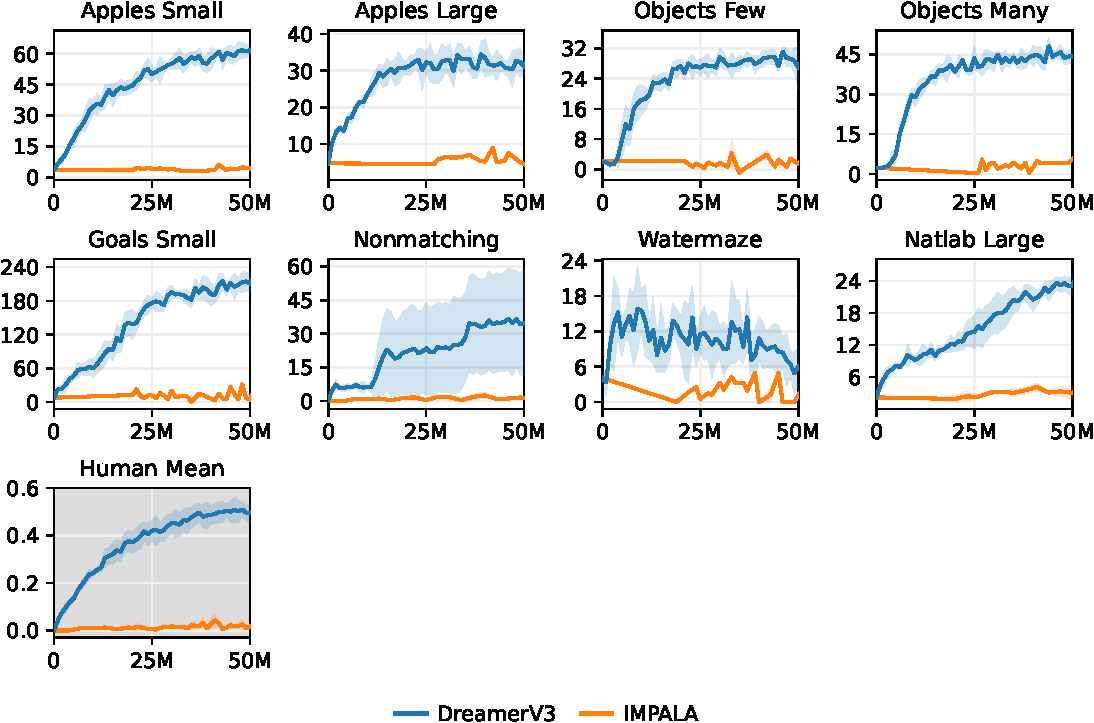
\includegraphics[width=1\linewidth]{dmlab/dmlab}
\caption{DMLab scores with a budget of 50M frames. Separate agents were trained for each task, corresponding to the IMPALA Experts method in \citet{espeholt2018impala}. Data efficiency is not the goal of IMPALA and it might be possible to tune it for improved data efficiency. Longer training curves and asymptotic performance of IMPALA are included in \cref{sec:dmlab_eff}.}
\label{fig:dmlab}
\end{figure}
\begin{table*}[h!]
\centering
\begin{mytabular}{
  colspec = {| L{8em} | C{8em} C{8em} C{8em} |},
  row{1} = {font=\bfseries},
}

\toprule
Task & DreamerV3 & IMPALA Steps & Ratio \\
\midrule
Goals Small & 214.7 & 8.0B & 80$\times$ \\
Goals Large & 68.1 & --- & $>$200$\times$ \\
Apples Small & 61.3 & 9.7B & 97$\times$ \\
Apples Large & 32.3 & 4.1B & 41$\times$ \\
Deferred Effects & 34.5 & --- & $>$200$\times$ \\
Keys Doors Puzzle & 27.6 & --- & $>$200$\times$ \\
Nonmatching & 34.3 & --- & $>$200$\times$ \\
Natlab Large & 23.1 & 3.7B & 37$\times$ \\
\bottomrule

\end{mytabular}
\caption{Data-efficiency comparison of DreamerV3 and IMPALA. The columns shows the score of DreamerV3 after 50M frames, how many steps IMPALA takes to reach the same score, and the resulting data-efficiency gain of DreamerV3 over IMPALA. The nonmatching task is excluded because DreamerV3 outperforms the final score of IMPALA here. The average efficiency gain across tasks is over 131.87$\times$}
\label{tab:dmlab_eff}
\end{table*}
\clearpage

\section{BSuite Scores}
\vspace{-2ex}
\begin{figure}[h]
\centering
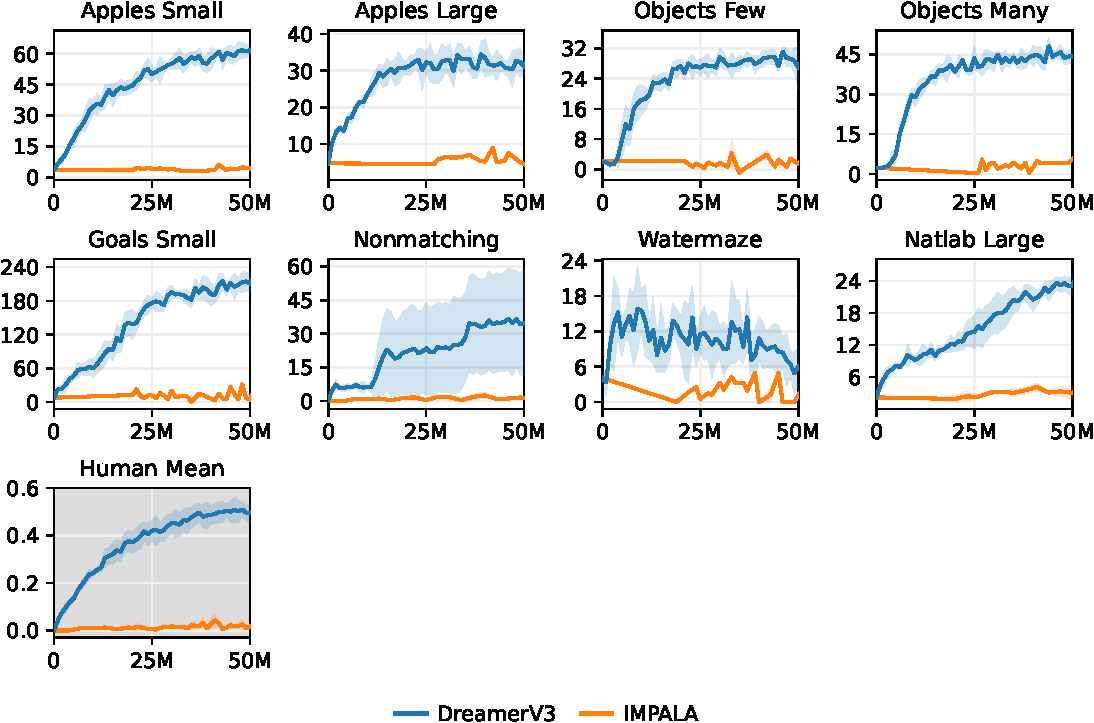
\includegraphics[width=1\linewidth]{dmlab/dmlab}
\caption{DMLab scores with a budget of 50M frames. Separate agents were trained for each task, corresponding to the IMPALA Experts method in \citet{espeholt2018impala}. Data efficiency is not the goal of IMPALA and it might be possible to tune it for improved data efficiency. Longer training curves and asymptotic performance of IMPALA are included in \cref{sec:dmlab_eff}.}
\label{fig:dmlab}
\end{figure}
\vspace{-2ex}
\begin{table}[h!]
\centering
\begin{mytabular}{
  colspec = {| L{11em} L{12.5em} | C{5.5em} | C{5.5em} |},
  row{1} = {font=\bfseries},
}

\toprule
Task & Categories & Muesli & \clap{DreamerV3} \\
\midrule
\texttt{bandit} & basic                                    & 0.908 & 0.859 \\
\texttt{bandit\_noise} & noise                             & 0.721 & 0.602 \\
\texttt{bandit\_scale} & scale                             & 0.674 & 0.680 \\
\texttt{cartpole} & basic, credit., generalization         & 0.906 & 0.853 \\
\texttt{cartpole\_noise} & noise, generalization           & 0.841 & 0.664 \\
\texttt{cartpole\_scale} & scale, generalization           & 0.701 & 0.779 \\
\texttt{cartpole\_swingup} & exploration, generalization   & 0.000 & 0.000 \\
\texttt{catch} & basic, credit assignment                  & 0.955 & 0.970 \\
\texttt{catch\_noise} & noise, credit assignment           & 0.464 & 0.571 \\
\texttt{catch\_scale} & scale, credit assignment           & 0.929 & 0.977 \\
\texttt{deep\_sea} & exploration                           & 0.000 & 0.000 \\
\texttt{deep\_sea\_stochastic} & exploration, noise        & 0.000 & 0.341 \\
\texttt{discounting\_chain} & credit assignment            & 0.453 & 0.290 \\
\texttt{memory\_len} & memory                              & 0.609 & 0.478 \\
\texttt{memory\_size} & memory                             & 0.706 & 0.706 \\
\texttt{mnist} & basic, generalization                     & 0.790 & 0.762 \\
\texttt{mnist\_noise} & noise, generalization              & 0.334 & 0.416 \\
\texttt{mnist\_scale} & scale, generalization              & 0.615 & 0.477 \\
\texttt{mountain\_car} & basic, generalization             & 0.797 & 0.949 \\
\texttt{mountain\_car\_noise} & noise, generalization      & 0.441 & 0.590 \\
\texttt{mountain\_car\_scale} & scale, generalization      & 0.400 & 0.948 \\
\texttt{umbrella\_distract} & credit assignment, noise     & 0.217 & 0.957 \\
\texttt{umbrella\_length} & credit assignment, noise       & 0.173 & 0.783 \\
\bottomrule
Category mean & & 0.537 & 0.627 \\
\bottomrule

\end{mytabular}
\caption{BSuite scores per environment averaged over environment configurations.}
\label{tab:bsuite}
\end{table}
\clearpage

\newgeometry{top=1.5cm,bottom=1.8cm,left=2.5cm,right=2.5cm}
\section{Crafter Scores}
\begin{figure}[h]
\centering
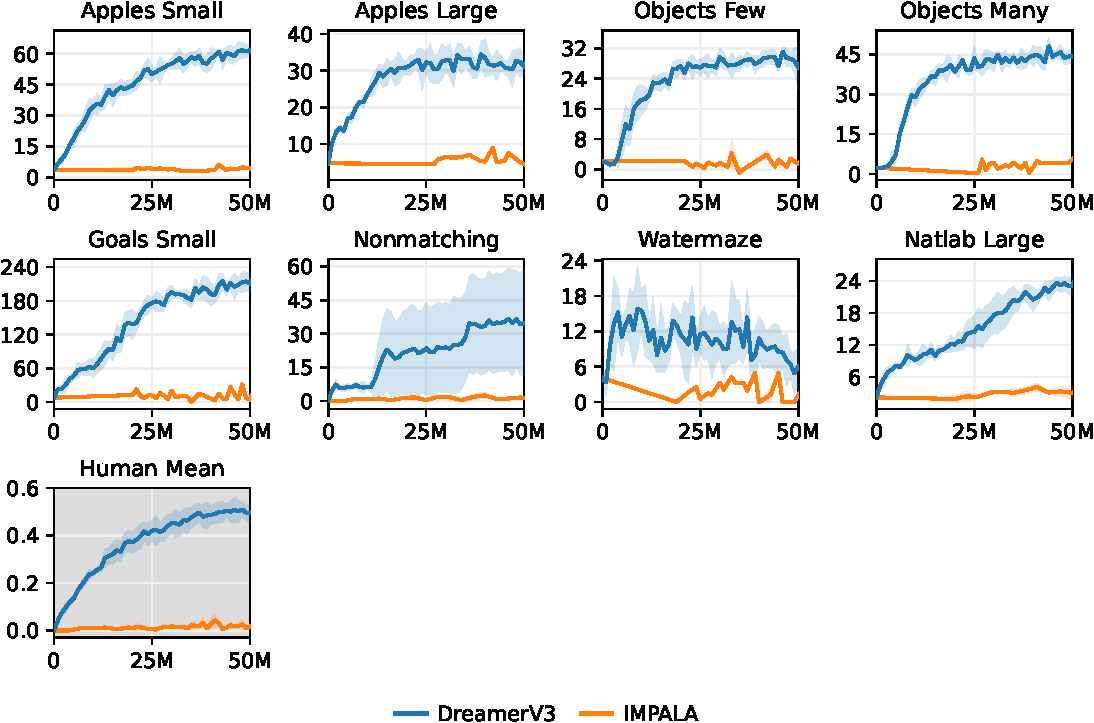
\includegraphics[width=1\linewidth]{dmlab/dmlab}
\caption{DMLab scores with a budget of 50M frames. Separate agents were trained for each task, corresponding to the IMPALA Experts method in \citet{espeholt2018impala}. Data efficiency is not the goal of IMPALA and it might be possible to tune it for improved data efficiency. Longer training curves and asymptotic performance of IMPALA are included in \cref{sec:dmlab_eff}.}
\label{fig:dmlab}
\end{figure}
\begin{table}[h!]
\centering
\begin{mytabular}{
  colspec = {| L{12em} | C{8em} C{8em} |},
  row{1} = {font=\bfseries},
}

\toprule
\textbf{Method} & \textbf{Score} & \textbf{Reward} \\
\midrule
Human Experts             & $ 50.5 \pm  6.8\%$ & $ 14.3 \pm  2.3$ \\
\midrule
DreamerV3                 & $\mathbf{14.5 \pm  1.6\%}$ & $\mathbf{11.7 \pm  1.9}$ \\
LSTM-SPCNN                & $ 12.1 \pm  0.8\%$ & --- \\
OC-SA                     & $ 11.1 \pm  0.7\%$ & --- \\
DreamerV2                 & $ 10.0 \pm  1.2\%$ & $\o9.0 \pm  1.7$ \\
PPO                       & $\o4.6 \pm  0.3\%$ & $\o4.2 \pm  1.2$ \\
Rainbow                   & $\o4.3 \pm  0.2\%$ & $\o6.0 \pm  1.3$ \\
Plan2Explore (Unsup)      & $\o2.1 \pm  0.1\%$ & $\o2.1 \pm  1.5$ \\
RND (Unsup)               & $\o2.0 \pm  0.1\%$ & $\o0.7 \pm  1.3$ \\
Random                    & $\o1.6 \pm  0.0\%$ & $\o2.1 \pm  1.3$ \\
\bottomrule

\end{mytabular}
\caption{Crafter scores compared to previous algorithms and human performance.}
\label{tab:crafter}
\end{table}

\restoregeometry
\clearpage

\section{Proprioceptive Control Curves}
\begin{figure}[h]
\centering
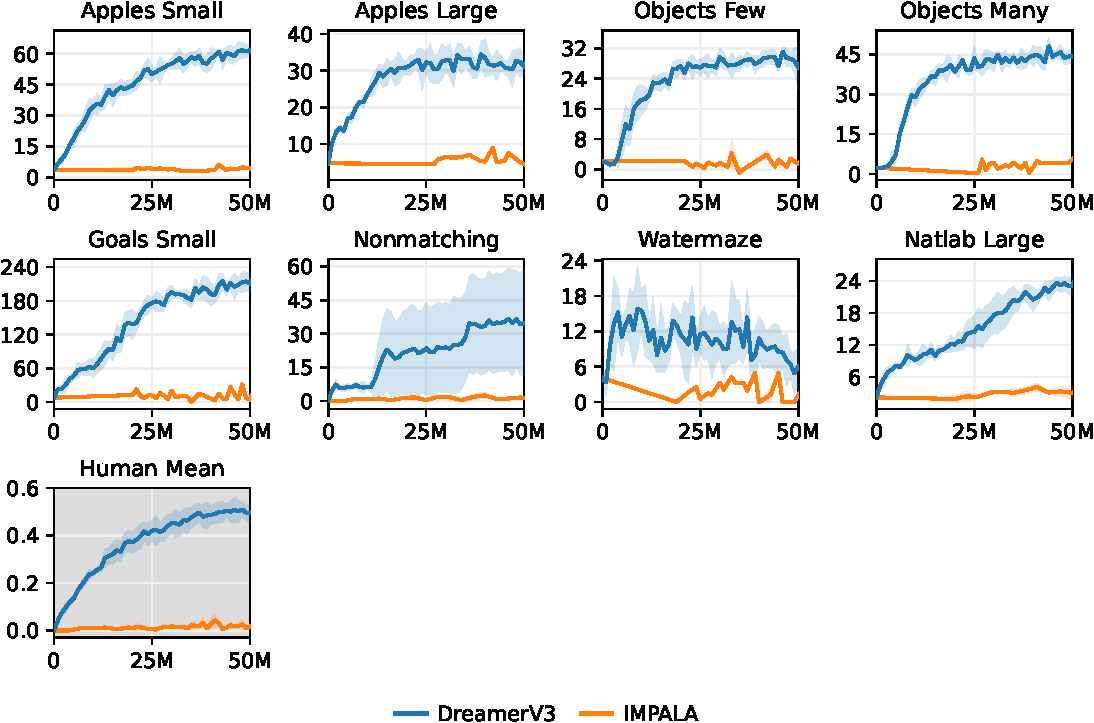
\includegraphics[width=1\linewidth]{dmlab/dmlab}
\caption{DMLab scores with a budget of 50M frames. Separate agents were trained for each task, corresponding to the IMPALA Experts method in \citet{espeholt2018impala}. Data efficiency is not the goal of IMPALA and it might be possible to tune it for improved data efficiency. Longer training curves and asymptotic performance of IMPALA are included in \cref{sec:dmlab_eff}.}
\label{fig:dmlab}
\end{figure}
\clearpage
\section{Proprioceptive Control Scores}
\begin{table*}[h!]
\centering
\begin{mytabular}{
  colspec = {| L{12em} | C{4em} C{4em} C{4em} C{4em} C{5em} |},
  row{1} = {font=\bfseries},
}

\toprule
Task & DDPG & MPO & DMPO & D4PG & DreamerV3 \\
\midrule
Environment Steps & 500K & 500K & 500K & 500K & 500K \\
\midrule
Acrobot Swingup & \o92.7 & \o80.6 & \o98.5 & 125.5 & \textbf{154.5} \\
Cartpole Balance & \textbf{996.2} & \textbf{958.4} & \textbf{998.5} & \textbf{998.8} & \textbf{990.5} \\
Cartpole Balance Sparse & \textbf{985.3} & \textbf{998.0} & \textbf{994.0} & \textbf{979.6} & \textbf{996.8} \\
Cartpole Swingup & \textbf{863.9} & \textbf{857.7} & \textbf{857.8} & \textbf{874.6} & \textbf{850.0} \\
Cartpole Swingup Sparse & 627.5 & 519.9 & 404.0 & \textbf{739.6} & 468.1 \\
Cheetah Run & 576.9 & \textbf{612.3} & 581.6 & \textbf{623.5} & 575.9 \\
Cup Catch & 905.5 & 800.6 & \textbf{965.8} & \textbf{968.3} & \textbf{958.2} \\
Finger Spin & 753.6 & 766.9 & 744.3 & 818.4 & \textbf{937.2} \\
Finger Turn Easy & 462.2 & 430.4 & 593.8 & 524.5 & \textbf{745.4} \\
Finger Turn Hard & 286.3 & 250.8 & 384.5 & 379.2 & \textbf{841.0} \\
Hopper Hop & \o24.6 & \o37.5 & \o71.5 & \o67.5 & \textbf{111.0} \\
Hopper Stand & 388.1 & 279.3 & 519.5 & \textbf{755.4} & 573.2 \\
Pendulum Swingup & 748.3 & \textbf{829.8} & \textbf{829.5} & 756.0 & 766.0 \\
Reacher Easy & \textbf{921.8} & \textbf{954.4} & \textbf{965.1} & \textbf{941.5} & \textbf{947.1} \\
Reacher Hard & \textbf{944.2} & \textbf{914.1} & \textbf{956.8} & \textbf{932.0} & \textbf{936.2} \\
Walker Run & 530.0 & 539.5 & 462.9 & 593.1 & \textbf{632.7} \\
Walker Stand & \textbf{967.4} & \textbf{960.4} & \textbf{971.6} & \textbf{935.2} & \textbf{956.9} \\
Walker Walk & \textbf{948.7} & \textbf{924.9} & \textbf{933.1} & \textbf{965.1} & \textbf{935.7} \\
\midrule
Median & 751.0 & 783.7 & 786.9 & 787.2 & \textbf{845.5} \\
Mean & 667.9 & 650.9 & 685.2 & 721.0 & \textbf{743.1} \\
\bottomrule

\end{mytabular}
\caption{DMC scores for proprioceptive inputs at 500K frames.}
\label{tab:dmc_proprio}
\end{table*}
\clearpage

\newgeometry{top=1.5cm,bottom=1cm,left=2.3cm,right=2.3cm}
\thispagestyle{blank}
\section{Visual Control Curves}
\begin{figure}[h]
\centering
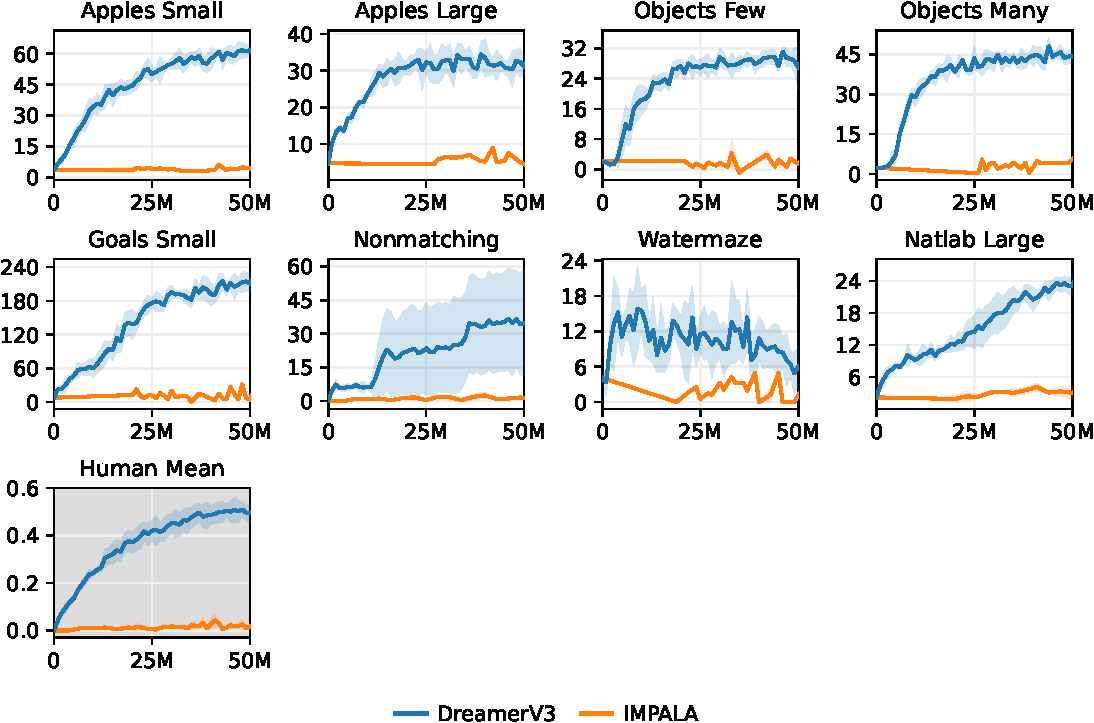
\includegraphics[width=1\linewidth]{dmlab/dmlab}
\caption{DMLab scores with a budget of 50M frames. Separate agents were trained for each task, corresponding to the IMPALA Experts method in \citet{espeholt2018impala}. Data efficiency is not the goal of IMPALA and it might be possible to tune it for improved data efficiency. Longer training curves and asymptotic performance of IMPALA are included in \cref{sec:dmlab_eff}.}
\label{fig:dmlab}
\end{figure}
\restoregeometry
\clearpage
\section{Visual Control Scores}
\begin{table*}[h!]
\centering
\begin{mytabular}{
  colspec = {| L{12em} | C{5em} C{5em} C{5em} C{5em} |},
  row{1} = {font=\bfseries},
}

\toprule
Task & SAC & CURL & DrQ-v2 & DreamerV3 \\
\midrule
Environment Steps & 1M & 1M & 1M & 1M \\
\midrule
Acrobot Swingup & \o\o5.1 & \o\o5.1 & 128.4 & \textbf{\o210.0} \\
Cartpole Balance & \textbf{963.1} & \textbf{979.0} & \textbf{991.5} & \textbf{\o996.4} \\
Cartpole Balance Sparse & \textbf{950.8} & \textbf{981.0} & \textbf{996.2} & \textbf{1000.0} \\
Cartpole Swingup & 692.1 & 762.7 & \textbf{858.9} & \textbf{\o819.1} \\
Cartpole Swingup Sparse & 154.6 & 236.2 & 706.9 & \textbf{\o792.9} \\
Cheetah Run & \o27.2 & 474.3 & 691.0 & \textbf{\o728.7} \\
Cup Catch & 163.9 & \textbf{965.5} & \textbf{931.8} & \textbf{\o957.1} \\
Finger Spin & 312.2 & \textbf{877.1} & \textbf{846.7} & \o818.5 \\
Finger Turn Easy & 176.7 & 338.0 & 448.4 & \textbf{\o787.7} \\
Finger Turn Hard & \o70.5 & 215.6 & 220.0 & \textbf{\o810.8} \\
Hopper Hop & \o\o3.1 & 152.5 & 189.9 & \textbf{\o369.6} \\
Hopper Stand & \o\o5.2 & 786.8 & \textbf{893.0} & \textbf{\o900.6} \\
Pendulum Swingup & 560.1 & 376.4 & \textbf{839.7} & \textbf{\o806.3} \\
Quadruped Run & \o50.5 & 141.5 & \textbf{407.0} & \o352.3 \\
Quadruped Walk & \o49.7 & 123.7 & \textbf{660.3} & \o352.6 \\
Reacher Easy & \o86.5 & 609.3 & \textbf{910.2} & \textbf{\o898.9} \\
Reacher Hard & \o\o9.1 & 400.2 & \textbf{572.9} & \o499.2 \\
Walker Run & \o26.9 & 376.2 & 517.1 & \textbf{\o757.8} \\
Walker Stand & 159.3 & 463.5 & \textbf{974.1} & \textbf{\o976.7} \\
Walker Walk & \o38.9 & 828.8 & 762.9 & \textbf{\o955.8} \\
\midrule
Median & 78.5 & 431.8 & 734.9 & \o\textbf{808.5} \\
Mean & 225.3 & 504.7 & 677.4 & \o\textbf{739.6} \\
\bottomrule

\end{mytabular}
\caption{DMC scores for visual inputs at 1M frames.}
\label{tab:dmc_vision}
\end{table*}
\clearpage

\section{Atari 100K Curves}
\begin{figure}[h]
\centering
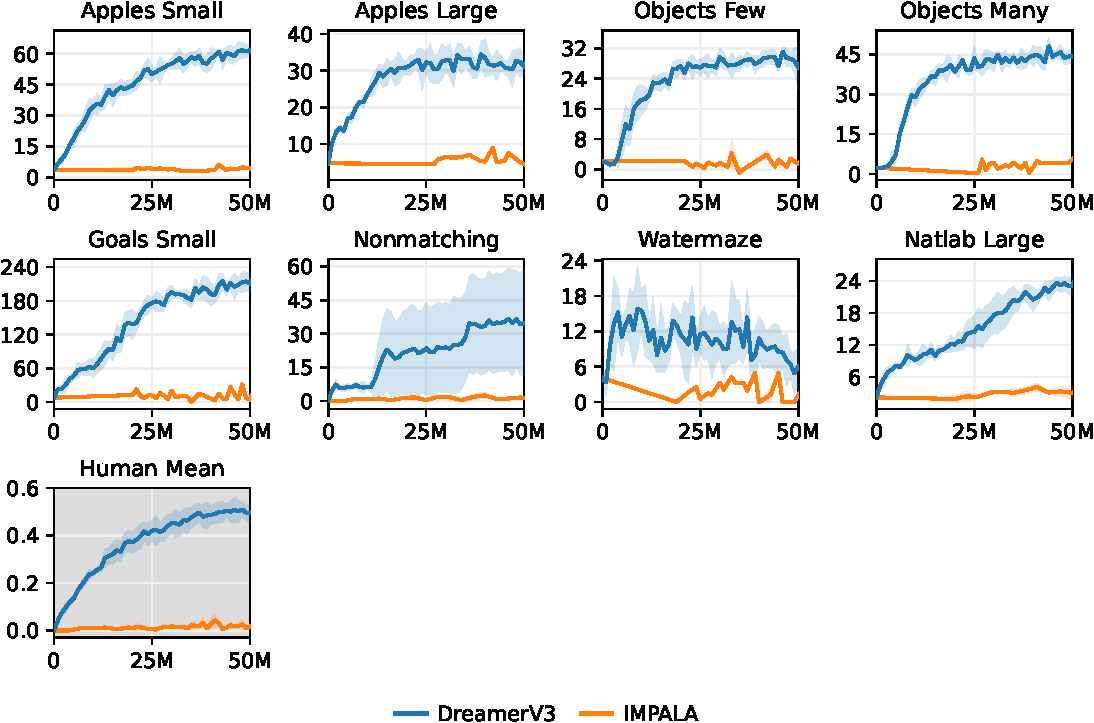
\includegraphics[width=1\linewidth]{dmlab/dmlab}
\caption{DMLab scores with a budget of 50M frames. Separate agents were trained for each task, corresponding to the IMPALA Experts method in \citet{espeholt2018impala}. Data efficiency is not the goal of IMPALA and it might be possible to tune it for improved data efficiency. Longer training curves and asymptotic performance of IMPALA are included in \cref{sec:dmlab_eff}.}
\label{fig:dmlab}
\end{figure}
\clearpage

\section{Atari 100K Scores}
\begin{table}[h!]
\begin{adjustwidth}{-10em}{-10em}
\centering
\begin{mytabular}{
  colspec = {| L{6.5em} | C{3.5em} C{3.5em} | C{4.5em} C{4.5em} C{4.5em} C{4.5em} C{4.5em} |},
  row{1} = {font=\bfseries},
  stretch = 0.8,
}

\toprule
Task & Random & Human & SimPLe & CURL & SPR & IRIS & \llap{Dr}eamerV3 \\
\midrule
Env Steps & --- & --- & --- & 400K & 400K & 400K & 400K \\
\midrule
Alien & \o\o228 & \o7128 & \o\o617 & \o711 & \o\o842 & \o\o420 & \textbf{\o\o959} \\
Amidar & \o\o\o\o6 & \o1720 & \o\o\o74 & \o114 & \textbf{\o\o180} & \o\o143 & \o\o139 \\
Assault & \o\o222 & \o\o742 & \o\o527 & \o501 & \o\o566 & \textbf{\o1524} & \o\o706 \\
Asterix & \o\o210 & \o8503 & \textbf{\o1128} & \o567 & \o\o962 & \o\o854 & \o\o932 \\
Bank Heist & \o\o\o14 & \o\o753 & \o\o\o34 & \o\o65 & \o\o345 & \o\o\o53 & \textbf{\o\o649} \\
Battle Zone & \o2360 & 37188 & \o4031 & 8998 & \textbf{14834} & 13074 & 12250 \\
Boxing & \o\o\o\o0 & \o\o\o12 & \o\o\o\o8 & \o\o\o1 & \o\o\o36 & \o\o\o70 & \textbf{\o\o\o78} \\
Breakout & \o\o\o\o2 & \o\o\o30 & \o\o\o16 & \o\o\o3 & \o\o\o20 & \textbf{\o\o\o84} & \o\o\o31 \\
Chopper Com. & \o\o811 & \o7388 & \o\o979 & \o784 & \o\o946 & \textbf{\o1565} & \o\o420 \\
Crazy Climber & 10780 & 35829 & 62584 & 9154 & 36700 & 59324 & \textbf{97190} \\
Demon Attack & \o\o152 & \o1971 & \o\o208 & \o646 & \o\o518 & \textbf{\o2034} & \o\o303 \\
Freeway & \o\o\o\o0 & \o\o\o30 & \o\o\o17 & \o\o28 & \o\o\o19 & \textbf{\o\o\o31} & \o\o\o\o0 \\
Frostbite & \o\o\o65 & \o4335 & \o\o237 & \textbf{1226} & \textbf{\o1171} & \o\o259 & \o\o909 \\
Gopher & \o\o258 & \o2412 & \o\o597 & \o401 & \o\o661 & \o2236 & \textbf{\o3730} \\
Hero & \o1027 & 30826 & \o2657 & 4988 & \o5859 & \o7037 & \textbf{11161} \\
James Bond & \o\o\o29 & \o\o303 & \o\o100 & \o331 & \o\o366 & \textbf{\o\o463} & \textbf{\o\o445} \\
Kangaroo & \o\o\o52 & \o3035 & \o\o\o51 & \o740 & \o3617 & \o\o838 & \textbf{\o4098} \\
Krull & \o1598 & \o2666 & \o2205 & 3049 & \o3682 & \o6616 & \textbf{\o7782} \\
Kung Fu Master & \o\o258 & 22736 & 14862 & 8156 & 14783 & \textbf{21760} & \textbf{21420} \\
Ms Pacman & \o\o307 & \o6952 & \textbf{\o1480} & 1064 & \o1318 & \o\o999 & \o1327 \\
Pong & \o\o\llap{--}21 & \o\o\o15 & \o\o\o13 & \o\llap{--}18 & \o\o\o\llap{--}5 & \o\o\o15 & \textbf{\o\o\o18} \\
Private Eye & \o\o\o25 & 69571 & \o\o\o35 & \o\o82 & \o\o\o86 & \o\o100 & \textbf{\o\o882} \\
Qbert & \o\o164 & 13455 & \o1289 & \o727 & \o\o866 & \o\o746 & \textbf{\o3405} \\
Road Runner & \o\o\o12 & \o7845 & \o5641 & 5006 & 12213 & \o9615 & \textbf{15565} \\
Seaquest & \o\o\o68 & 42055 & \textbf{\o\o683} & \o315 & \o\o558 & \textbf{\o\o661} & \o\o618 \\
\midrule
Human Median & 0\rlap{\%} & 100\rlap{\%} & 13\rlap{\%} & \o9\rlap{\%} & 40\rlap{\%} & \o29\rlap{\%} & \textbf{\o49\rlap{\%}} \\
Human Mean & 0\rlap{\%} & 100\rlap{\%} & 33\rlap{\%} & 26\rlap{\%} & 62\rlap{\%} & 105\rlap{\%} & \textbf{112\rlap{\%}} \\
\bottomrule

\end{mytabular}
\end{adjustwidth}
\vspace{-0.5ex}
\caption{Atari scores at 400K environment frames, corresponding to 100k agent frames.}
\label{tab:atari100k}
\end{table}

\clearpage

\section{Atari 100K Settings}
\begin{table}[h!]
\begin{adjustwidth}{-10em}{-10em}
\centering
\begin{mytabular}{
  colspec = {| L{10em} | C{4.5em} C{4.5em} C{4.5em} C{4.5em} C{4.5em} C{4.5em} |},
  row{1} = {font=\bfseries},
}

\toprule
Setting & SimPLe & \clap{EfficientZero} & SPR & IRIS & TWM & \llap{Dr}eamerV3 \\
\midrule
Mean score   & 33 & 190 & 70 & 104 & 95 & 112 \\
Median score & 13 & 109 & 41 & 29 & 50 & 49 \\
GPU days     & 10 & 1.2 & 0.2 & 7 & 0.8 & 0.5 \\
\midrule
Online planning        & --- &  X  & --- & --- & --- & --- \\
Data augmentation      & --- & --- &  X  & --- & --- & --- \\
Non-uniform replay     & --- &  X  &  X  & --- &  X  & --- \\
Separate hparams       & --- & --- & --- &  X  & --- & --- \\
Increased resolution   & --- &  X  &  X  & --- & --- & --- \\
Uses life information  & --- &  X  &  X  &  X  &  X  & --- \\
Uses early resets      & --- &  X  & --- &  X  & --- & --- \\
Separate eval episodes &  X  &  X  &  X  &  X  &  X  & --- \\
\bottomrule

\end{mytabular}
\end{adjustwidth}
\vspace{-0.5ex}
\caption{Algorithmic components, algorithmic components, and environment settings for the Atari 100k benchmark. GPU days are converted to V100 days by assuming P100 is twice as slow and A100 is twice as fast. EfficientZero achieves the highest scores but at the cost of complexity and changing the environment configuration. IRIS uses a separate exploration strength for Freeway.}
\label{tab:atari100k_setting}
\end{table}

\clearpage

\newgeometry{top=1cm,bottom=1cm,left=2.3cm,right=2.3cm}
\thispagestyle{blank}
\section{Atari 200M Curves}
\vspace{-2ex}
\begin{figure}[h]
\centering
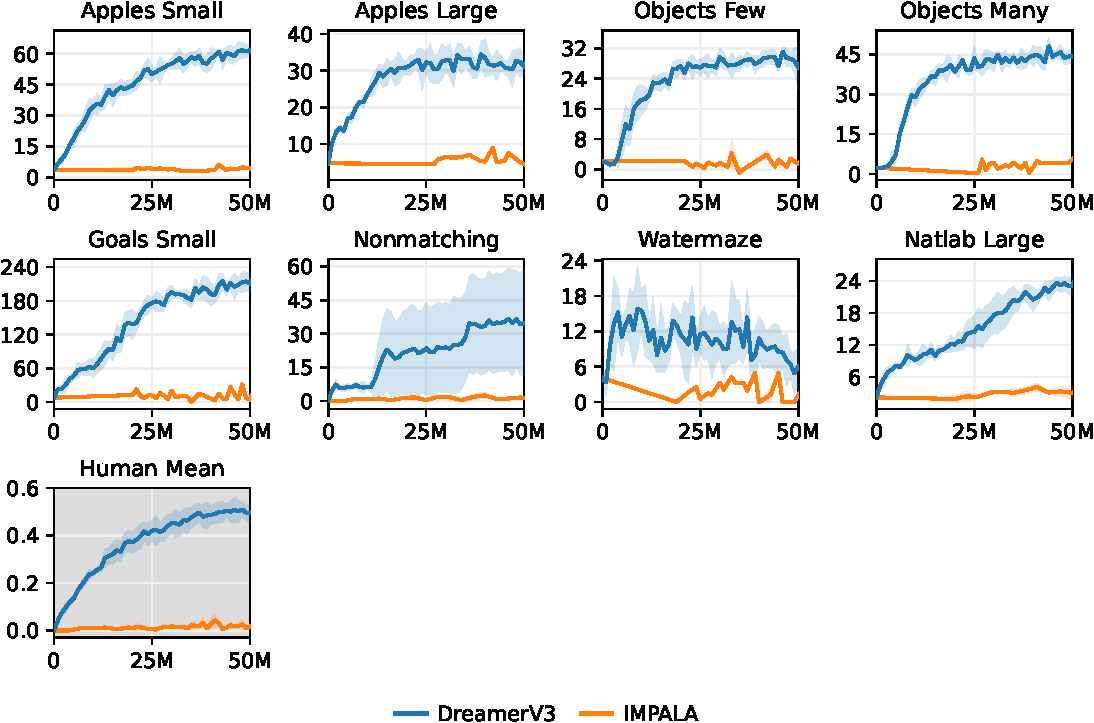
\includegraphics[width=1\linewidth]{dmlab/dmlab}
\caption{DMLab scores with a budget of 50M frames. Separate agents were trained for each task, corresponding to the IMPALA Experts method in \citet{espeholt2018impala}. Data efficiency is not the goal of IMPALA and it might be possible to tune it for improved data efficiency. Longer training curves and asymptotic performance of IMPALA are included in \cref{sec:dmlab_eff}.}
\label{fig:dmlab}
\end{figure}
\clearpage
\thispagestyle{blank}
\section{Atari 200M Scores}
\vspace{-1ex}
\begin{table}[h!]
\begin{adjustwidth}{-10em}{-10em}
\centering\small
\begin{mytabular}{
  colspec = {| L{8.5em} | C{4em} C{4em} C{4em} | C{4.8em} C{4.8em} C{4.8em} C{4.8em} |},
  row{1} = {font=\bfseries},
  stretch = 0.8,
}

\toprule
Task & Random & Gamer & Record & IQN & Rainbow & DreamerV2 & DreamerV3 \\
\midrule
Environment Steps & --- & --- & --- & 200M & 200M & 200M & 200M \\
\midrule
Alien & \o\o229 & \o7128 & \o\o251916 & \o\o4926 & \o\o3488 & \o\o4083 & \textbf{\o\o\o5404} \\
Amidar & \o\o\o\o6 & \o1720 & \o\o104159 & \o\o2315 & \textbf{\o\o2530} & \textbf{\o\o2531} & \o\o\o1141 \\
Assault & \o\o222 & \o\o742 & \o\o\o\o8647 & \o\o4639 & \o\o3302 & \textbf{\o23504} & \o\o18876 \\
Asterix & \o\o210 & \o8503 & \o1000000 & \o10293 & \o17534 & \textbf{\o75598} & \o\o39643 \\
Asteroids & \o\o719 & 47389 & 10506650 & \o\o1578 & \o\o1468 & \textbf{\o40120} & \o\o\o3829 \\
Atlantis & 12850 & 29028 & 10604840 & 890427 & 790051 & 996300 & \textbf{1439392} \\
Bank Heist & \o\o\o14 & \o\o753 & \o\o\o82058 & \o\o1056 & \textbf{\o\o1079} & \textbf{\o\o1127} & \o\o\o1000 \\
Battle Zone & \o2360 & 37188 & \o\o801000 & \textbf{\o40784} & \textbf{\o40194} & \textbf{\o42210} & \o\o35912 \\
Beam Rider & \o\o364 & 16926 & \o\o999999 & \o\o7042 & \o\o6232 & \o18157 & \textbf{\o\o20051} \\
Berzerk & \o\o124 & \o2630 & \o1057940 & \o\o\o644 & \o\o\o822 & \o\o\o807 & \textbf{\o\o\o1245} \\
Bowling & \o\o\o23 & \o\o161 & \o\o\o\o\o300 & \o\o\o\o39 & \o\o\o\o39 & \o\o\o\o49 & \textbf{\o\o\o\o158} \\
Boxing & \o\o\o\o0 & \o\o\o12 & \o\o\o\o\o100 & \textbf{\o\o\o\o98} & \textbf{\o\o\o\o98} & \o\o\o\o91 & \textbf{\o\o\o\o\o99} \\
Breakout & \o\o\o\o2 & \o\o\o30 & \o\o\o\o\o864 & \o\o\o\o80 & \o\o\o109 & \textbf{\o\o\o293} & \textbf{\o\o\o\o300} \\
Centipede & \o2091 & 12017 & \o1301709 & \o\o3735 & \o\o6538 & \o11816 & \textbf{\o240525} \\
Chopper Com. & \o\o811 & \o7388 & \o\o999999 & \o\o9106 & \textbf{\o12388} & \o\o2647 & \o\o\o5853 \\
Crazy Climber & 10780 & 35829 & \o\o219900 & 134761 & 145889 & \textbf{158278} & \o149986 \\
Demon Attack & \o\o152 & \o1971 & \o1556345 & \o14558 & \o16049 & \textbf{\o84408} & \o\o77084 \\
Double Dunk & \o\o\llap{--}19 & \o\o\llap{--}16 & \o\o\o\o\o\o22 & \o\o\o\o21 & \textbf{\o\o\o\o22} & \o\o\o\o18 & \textbf{\o\o\o\o\o23} \\
Enduro & \o\o\o\o0 & \o\o860 & \o\o\o\o9500 & \textbf{\o\o2207} & \textbf{\o\o2181} & \o\o1775 & \textbf{\o\o\o2289} \\
Fishing Derby & \o\o\llap{--}92 & \o\o\llap{--}39 & \o\o\o\o\o\o71 & \o\o\o\o44 & \o\o\o\o42 & \o\o\o\o66 & \textbf{\o\o\o\o\o77} \\
Freeway & \o\o\o\o0 & \o\o\o30 & \o\o\o\o\o\o38 & \textbf{\o\o\o\o34} & \textbf{\o\o\o\o34} & \textbf{\o\o\o\o33} & \textbf{\o\o\o\o\o34} \\
Frostbite & \o\o\o65 & \o4335 & \o\o454830 & \o\o7866 & \o\o8351 & \o12091 & \textbf{\o\o19991} \\
Gopher & \o\o258 & \o2412 & \o\o355040 & \o11469 & \o10272 & \textbf{\o91249} & \textbf{\o\o86759} \\
Gravitar & \o\o173 & \o3351 & \o\o162850 & \o\o1332 & \o\o1263 & \textbf{\o\o3769} & \o\o\o\o560 \\
Hero & \o1027 & 30826 & \o1000000 & \o36216 & \textbf{\o46417} & \o22003 & \o\o35359 \\
Ice Hockey & \o\o\llap{--}11 & \o\o\o\o1 & \o\o\o\o\o\o36 & \o\o\o\o\llap{--}5 & \o\o\o\o\llap{--}0 & \textbf{\o\o\o\o26} & \textbf{\o\o\o\o\o27} \\
Jamesbond & \o\o\o\o7 & \o\o303 & \o\o\o45550 & \o\o3294 & \o\o1035 & \textbf{\o38514} & \o\o\o5123 \\
Kangaroo & \o\o\o52 & \o3035 & \o1424600 & \o12562 & \o12812 & \textbf{\o13899} & \o\o11597 \\
Krull & \o1598 & \o2666 & \o\o104100 & \o\o8771 & \o\o4238 & \textbf{\o55217} & \o\o20123 \\
Kung Fu Master & \o\o258 & 22736 & \o1000000 & \o30431 & \o26489 & \o63614 & \textbf{\o\o68166} \\
Montezuma Rev. & \o\o\o\o0 & \o4753 & \o1219200 & \o\o\o495 & \o\o\o487 & \o\o\o\o79 & \textbf{\o\o\o2512} \\
Ms Pacman & \o\o307 & \o6952 & \o\o290090 & \o\o5153 & \o\o3913 & \o\o5693 & \textbf{\o\o11397} \\
Name This Game & \o2292 & \o8049 & \o\o\o25220 & \o\o6718 & \o\o9073 & \o14879 & \textbf{\o\o26439} \\
Phoenix & \o\o761 & \o7243 & \o4014440 & \o\o5098 & \o\o8355 & \o47024 & \textbf{\o\o90037} \\
Pitfall & \o\llap{--}229 & \o6464 & \o\o114000 & \o\o\o\llap{--}17 & \o\o\o\llap{--}12 & \o\o\o\o\llap{--}2 & \o\o\o\o\o\llap{--}0 \\
Pong & \o\o\llap{--}21 & \o\o\o15 & \o\o\o\o\o\o21 & \textbf{\o\o\o\o20} & \textbf{\o\o\o\o20} & \textbf{\o\o\o\o20} & \textbf{\o\o\o\o\o20} \\
Private Eye & \o\o\o25 & 69571 & \o\o101800 & \o\o4286 & \textbf{\o21341} & \o\o2073 & \o\o\o5538 \\
Qbert & \o\o164 & 13455 & \o2400000 & \o16464 & \o17625 & 114114 & \textbf{\o137224} \\
Riverraid & \o1338 & 17118 & \o1000000 & \o15250 & \textbf{\o20766} & \o16791 & \o\o15758 \\
Road Runner & \o\o\o12 & \o7845 & \o2038100 & \o58813 & \o54704 & \textbf{249230} & \o\o78005 \\
Robotank & \o\o\o\o2 & \o\o\o12 & \o\o\o\o\o\o76 & \o\o\o\o66 & \o\o\o\o65 & \textbf{\o\o\o\o77} & \o\o\o\o\o66 \\
Seaquest & \o\o\o68 & 42055 & \o\o999999 & \o16819 & \o\o9966 & \o\o7341 & \textbf{\o\o49547} \\
Skiing & \llap{--}17098 & \llap{--}4337 & \o\o\o\llap{--}3272 & \llap{--}11156 & \llap{--}28322 & \o\llap{--}9813 & \o\o\llap{--}9623 \\
Solaris & \o1236 & 12327 & \o\o111420 & \o\o1659 & \o\o1829 & \o\o1016 & \textbf{\o\o\o2453} \\
Space Invaders & \o\o148 & \o1669 & \o\o621535 & \o\o4562 & \o\o4112 & \o\o2615 & \textbf{\o\o\o6269} \\
Star Gunner & \o\o664 & 10250 & \o\o\o77400 & \textbf{\o79330} & \o57289 & \o10908 & \o\o\o8423 \\
Tennis & \o\o\llap{--}24 & \o\o\o\llap{--}8 & \o\o\o\o\o\o21 & \textbf{\o\o\o\o23} & \o\o\o\o\llap{--}0 & \o\o\o\o14 & \textbf{\o\o\o\o\o23} \\
Time Pilot & \o3568 & \o5229 & \o\o\o65300 & \o11619 & \o12041 & \o36059 & \textbf{\o\o68980} \\
Tutankham & \o\o\o11 & \o\o168 & \o\o\o\o5384 & \o\o\o248 & \o\o\o240 & \o\o\o265 & \textbf{\o\o\o\o285} \\
Up N Down & \o\o533 & 11693 & \o\o\o82840 & \o63430 & \o35440 & \textbf{651439} & \o502213 \\
Venture & \o\o\o\o0 & \o1188 & \o\o\o38900 & \o\o1314 & \textbf{\o\o1539} & \o\o\o\o\o0 & \o\o\o\o\o\o0 \\
Video Pinball & 16257 & 17668 & 89218328 & 420509 & \textbf{450968} & \o46282 & \o\o17416 \\
Wizard Of Wor & \o\o564 & \o4756 & \o\o395300 & \o\o5595 & \o\o7869 & \o12396 & \textbf{\o\o36537} \\
Yars Revenge & \o3093 & 54577 & 15000105 & \o83990 & \o45059 & 157285 & \textbf{\o235402} \\
Zaxxon & \o\o\o32 & \o9173 & \o\o\o83700 & \o11047 & \o14606 & \textbf{\o48620} & \o\o36626 \\
\midrule
Gamer Median & 0\rlap{\%} & 100\rlap{\%} & \o\o3716\rlap{\%} & 126\rlap{\%} & 147\rlap{\%} & \o219\rlap{\%} & \textbf{302\rlap{\%}} \\
Gamer Mean & 0\rlap{\%} & 100\rlap{\%} & 126759\rlap{\%} & 890\rlap{\%} & 888\rlap{\%} & \textbf{1149\rlap{\%}} & 920\rlap{\%} \\
Record Mean & 0\rlap{\%} & \o12\rlap{\%} & \o\o\o100\rlap{\%} & \o21\rlap{\%} & \o17\rlap{\%} & \textbf{\o\o44\rlap{\%}} & \o41\rlap{\%} \\
Clip Record Mean & 0\rlap{\%} & \o12\rlap{\%} & \o\o\o100\rlap{\%} & \o21\rlap{\%} & \o17\rlap{\%} & \textbf{\o\o28\rlap{\%}} & \textbf{\o29\rlap{\%}} \\
\bottomrule

\end{mytabular}
\end{adjustwidth}
\vspace*{-1ex}
\caption{Atari scores at 200M frames.}
\label{tab:atari}
\vspace*{-3ex}
\end{table}

\restoregeometry
\clearpage

\section{Hyperparameters}
\begin{table}[h!]
\centering
\begin{mytabular}{
  colspec = {| L{15em} | C{6em} | C{10em} |},
  row{1} = {font=\bfseries},
}

\toprule
\textbf{Name} & \textbf{Symbol} & \textbf{Value} \\
\midrule
\multicolumn{3}{l}{\textbf{General}} \\
\midrule
Replay capacity (FIFO) & --- & $10^6\!\!$ \\
Batch size & $B$ & 16 \\
Batch length & $T$ & 64 \\
Activation & --- & $\operatorname{LayerNorm}+\operatorname{SiLU}$ \\
\midrule
\multicolumn{3}{l}{\textbf{World Model}} \\
\midrule
Number of latents & --- & 32 \\
Classes per latent & --- & 32 \\
Reconstruction loss scale & $\beta_{\mathrm{pred}}$ & 1.0 \\
Dynamics loss scale & $\beta_{\mathrm{dyn}}$ & 0.5 \\
Representation loss scale & $\beta_{\mathrm{rep}}$ & 0.1 \\
Learning rate & --- & $10^{-4}$ \\
Adam epsilon & $\epsilon$ & $10^{-8}$ \\
Gradient clipping & --- & 1000 \\
\midrule
\multicolumn{3}{l}{\textbf{Actor Critic}} \\
\midrule
Imagination horizon & $H$ & 15 \\
Discount horizon & $1/(1-\gamma)$ & 333 \\
Return lambda & $\lambda$ & 0.95 \\
Critic EMA decay & --- & 0.98 \\
Critic EMA regularizer & --- & 1 \\
Return normalization scale & $S$ & $\operatorname{Per}(R, 95) - \operatorname{Per}(R, 5)$ \\
Return normalization limit & $L$ & 1 \\
Return normalization decay & --- & 0.99 \\
Actor entropy scale & $\eta$ & $3\cdot10^{-4}$ \\
Learning rate & --- & $3\cdot10^{-5}$ \\
Adam epsilon & $\epsilon$ & $10^{-5}$ \\
Gradient clipping & --- & 100 \\
\bottomrule

\end{mytabular}
\caption{DreamerV3 hyper parameters. The same values are used across all benchmark suites, including proprioceptive and visual inputs, continuous and discrete actions, and 2D and 3D domains. We do not use any hyperparameter annealing, weight decay, or dropout.
}
\label{tab:hparams}
\end{table}

